\documentclass[letterpaper,11pt,twoside]{article}
\usepackage{amsmath,amssymb,amsfonts,amsthm}
\usepackage[margin=1.0in]{geometry}
\usepackage{fancyhdr, lastpage}
\usepackage[pdftex]{graphicx}
\usepackage{hyperref}
\hypersetup{
    colorlinks,
    citecolor={black},
    linkcolor={black},
    urlcolor={black},
    bookmarksnumbered,
    pdfstartview={FitH},
    pdfpagemode={UseOutlines},
    pdftitle={Project Report - Distributed Query Processing},
    pdfauthor={Larry Bowers, James Bradwell, Evan Dickinson, Bhadresh Patel, and Lewis Pearson},
    pdfsubject={CS 453 Project Report}
}

\setlength{\parskip}{0.5ex}
\pagestyle{fancy}
\setlength{\headheight}{14.0pt}
\fancyhead{}
\fancyfoot{}
\fancyhead[RO,RE] {Project Report: \emph{Distributed Query Processing}}
\fancyfoot[LO,LE] {CS 453: Project 4}
\fancyfoot[RO,RE] {Page \thepage\ of \pageref{LastPage}}
\renewcommand{\headrulewidth}{0.5pt}
\renewcommand{\footrulewidth}{0.5pt}

\begin{document}

%%%%%%%%%% Title Page %%%%%%%%%%%%%%%%%%%%%%%%%%%%%%%%%%%%%%%%%%%%%%%%%%%%%%%%%%
\begin{titlepage}
   \begin{center}
       {\Large \textbf{Project Report}}\\[0.5cm]
       {\Large \textbf{CS 453: Project 4}}\\[3.0cm]

       {\rule{\linewidth}{0.5mm}} \\[0.5cm]
       {\Huge \textbf{Distributed Query Processing}}\\[0.4cm] 
       {\rule{\linewidth}{0.5mm}} \\[2.0cm]

       \textbf{Larry Bowers}\\
       \texttt{killergift@wsu.edu}\\[0.5cm]
       \textbf{James Bradwell}\\
       \texttt{jebradwell@gmail.com}\\[0.5cm]
       \textbf{Evan Dickinson}\\
       \texttt{evan13579b@wsu.edu}\\[0.5cm]
       \textbf{Bhadresh Patel}\\
       \texttt{bhadresh@wsu.edu}\\[0.5cm]
       \textbf{Lewis Pearson}\\
       \texttt{lewis\_pearson@wsu.edu}\\[0.5cm]

       \vfill
       Washington State University Vancouver\\
       December 05, 2010
   \end{center}
\end{titlepage}

\begin{abstract}
The main goal of this project is to provide user interface for the search engine and process user's query over multiple Amazon EC2 nodes using the PageRank and Indexes generated by previous project.
\end{abstract}

\section{Overview}

\begin{figure}[htb]
 \centering
 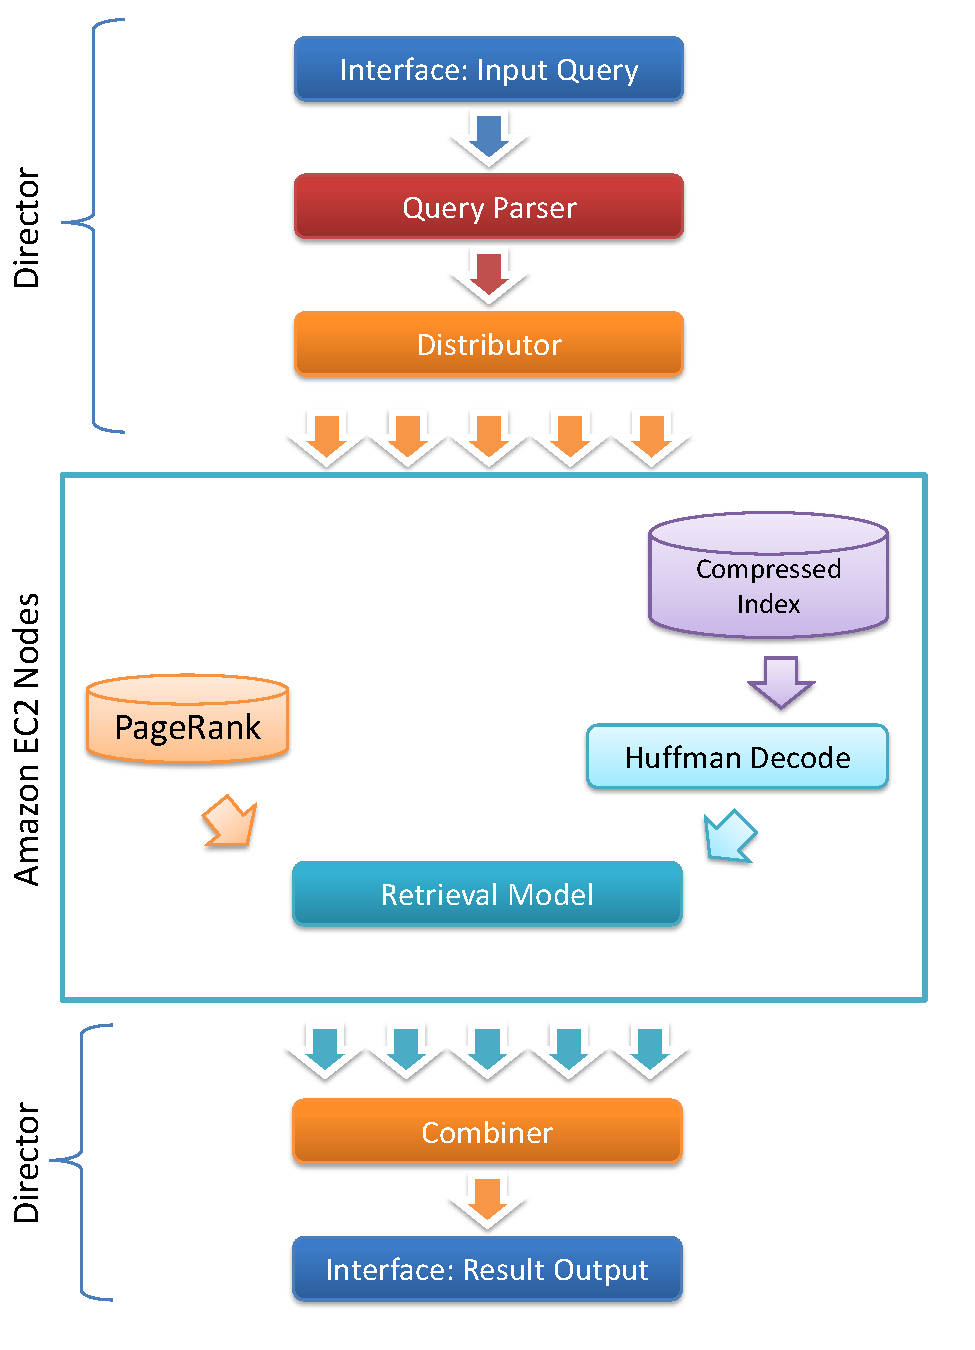
\includegraphics[trim=0.0in 0.00in 0.0in 0.0in, clip, page=1]{Architecture.pdf}
 \caption{Architecture Overview}
 \label{fig:Architecture}
\end{figure}

\section{Interface}

\subsection{Query Input}

\subsection{Result Output}

\section{Distributed Evaluation}

\subsection{Distributer}

\subsection{Index Server}

\subsection{Merge Results}

\section{Index Compression}

\section{Retrieval Model}

\subsection{Query Likelihood}

\subsection{BM25}

\section{Roles}
\begin{description}
  \item[Larry Bowers] User interface and query parser
  \item[James Bradwell] User interface and query parser
  \item[Evan Dickinson] Huffman encoding/decoding 
  \item[Bhadresh Patel] Distributed evaluation
  \item[Lewis Pearson] Retrieval model
\end{description}

\section{Test Environment}

For testing/production purpose, we have set up instances on Amazon EC2. The instance id of the director machine is i-5135773c which also hosts the user interface. Instance ids of five index servers are: (i) i-5335773e, (ii) i-2d357740, (iii) i-2f357742, (iv) i-29357744, and (v) i-2b357746. The source code on all instances is checked out at /home/ubuntu/dqp/. The user interface can be accessed via public DNS name of the director instance. For example, http://ec2-174-129-159-24.compute-1.amazonaws.com/ui/.

\section{Usage Guide}

\begin{itemize}
	\item Update Nodes file \texttt{dp/local.nodes} or \texttt{dp/cloud.nodes}. Change the IP address of all nodes for the appropriate environment.
	\item Start index server on each instance
\begin{verbatim}
	$ python ~/dqp/dp/server.py
\end{verbatim}
	\item Find the public DNS of the director instance \texttt{i-5135773c}. Launch the UI using public DNS, for example, http://ec2-174-129-159-24.compute-1.amazonaws.com/ui/.
\end{itemize}


\end{document}
